\documentclass[11pt]{article}

\usepackage[backend=bibtex]{biblatex}
\usepackage[utf8]{inputenc}
\usepackage{amsmath}
\usepackage{amssymb}
\usepackage{anysize}
\usepackage{graphicx}
\usepackage{subcaption}
\graphicspath{ {./images/}, {./parts/igor/}, {./parts/igor/images/} }
\usepackage{color}
\usepackage{xcolor}
\usepackage{algorithm2e}
\usepackage{pgfplots}
\usepackage{hyperref}
\usepackage{booktabs}
\usepackage{tabularx}
\usepackage{titlesec}
\usepackage{array}
\usepackage{listings}
\bibliography{bibliography.bib}

\usepackage{tikz}
\usetikzlibrary{shapes,arrows, trees}

\definecolor{mygreen}{rgb}{0,0.6,0}
\definecolor{mygray}{rgb}{0.5,0.5,0.5}
\definecolor{mypurple}{rgb}{0.58,0,0.82}


\usepackage{caption}
\DeclareCaptionFont{white}{\color{white}}
\DeclareCaptionFormat{listing}{\colorbox{gray}{\parbox[c]{\textwidth}{#1#2#3}}}

\setlength\parindent{0pt}
\setlength{\parskip}{10pt}

\marginsize{2cm}{2cm}{1cm}{1cm}
% % % % % % % % % % % % % % % % % % % % % % % % % % % % % % % % % % % % % %
% % % Commands
\titleformat{\paragraph}
{\normalfont\normalsize\bfseries\space}
{}
{0pt}
{}

% % % % % % % % % % % % % % % % % % % % % % % % % % % % % % % % % % % % % %
% % % Document start
\begin{document}

%  Title and authors
   \begin{center}
     {\huge\bfseries B31XP Robotics project\\ Robotic object follower}\\
      \vspace{2ex}
      \textsc{Andrey Pak, Donatas Kozlovskis, Enric Cornellà,\\ Fernando Garcia,  Igor Peric}
   \end{center}
   \vspace{2ex}%

%  Abstract
\begin{abstract}
This project presents a small, easy to build low-cost robot system, that is able to find coloured signs on the floor and implement the associated actions, e.g. stop, turn, pause, etc.
The robot hardware uses Raspberry Pi to control a set of motors, sensors and servo actuators. 
This report provides review of the hardware design and implementation of software using open source tools as C++ and OpenCV libraries. 
\end{abstract}

\section{Introduction}
\label{sec:intro}

Nowadays automation and robotics are leaving the traditional sectors as industrial manufacturing and becoming a part of daily life. It is integrating into our society, while many members still do not have a knowledge of it, since they are only familiar with the form of automation learned from massive social media.
Because of this trend of automation, it is important that educational organizations start preparing not only robotic researchers and designers, but also industrial personnel, who will be able
to take care of the robotic devices existing in our daily environment. 

A broad variety of robotic courses offered by universities or by massive open online education systems, increased during the past several years. However young students still lack opportunities to get hands-on experience on the understanding working principles, fabrication and implementation of robotic devices, which leads to the gap between theoretical and practical domain knowledge.

This project covered developing a low-cost wheeled robot, which is intended to promoting the teaching of basic computer science in schools \footnote{\url{http://www.raspberrypi.org/picademy/}}. Initial hardware design was provided by project supervisor, with limitations of only having motor servos, distance sensor, LCD screen, camera and Raspberry Pi (RPi) single-board computer.
Constraint of  Raspberry Pi computation power raised challenge to find an  optimal techniques of implementing controllers of sensors and actuators, knowing that the most of resources are consumed by image processing to implement and realise desired robot actions. Here, the optimal software design procedure is presented leading to the working example of constructed robot.


\section{Description of the Project}
The present section describes the different stages of the project; design, management, software implementation and hardware improvement. It also presents the main goals of the work as well as a brief description of the main sections which compose this document.

As it has been presented in section \ref{sec:intro}, the main goal of the project is to introduce robotics in general and open-source tools such as Raspberry Pi in a dynamic and friendly manner in order to enhance the learning experience and engage children. It has been proved that the most suitable way to achieve this is to present the activity as an interactive game \cite{bransford1999people}.

Considering the importance of self-motivation in whatever successful learning process, it is important to assure an enjoyable experience for the user, conditioned by the field studied. For this reason this topic is worth it to be studied.

The main goal is to provide an independent robot platform able to interact with the user, in this case children. This idea not only forces the implementation to be as robust as possible, but also it forces to implement a strong feedback component in order to give the impression to the user what is going on at every single moment during the game development. It is so important to assure the reduction of uncertainty moments produced by an expected reaction of the system as well as a lack of information during the actions performed. 

Firstly, and according to the previous statement, a robust interaction method needs to be defined because it will provide to the user the control of the system in a reliable way. An intuitive technique to do this is to make the robot able to recognize different signs and execute the correspondent actions when one of these signs are presented. The basic signs are an arrow, a cross and a circle but it can be easily extended to more. Showing this bunch of signs to the platform, children should be able to give the appropriate instructions to move it from point A to point B.

Secondly, the concept of feedback in every single moment is essential. It will provide the current state of the process, reinforcement or additional guidance to continue the experience. In this way, two different types of feedback are defined: acoustic and visual. 

The first type of feedback is provided using a set of representative sounds indicating robot start and stop of the program (game). The second type of feedback is provided through text displayed in a LCD screen guiding the user in any situation.

The main challenge of this project is to be able to segment the sign properly under different lighting conditions and surfaces, but also taking into account the limited computational power of the Raspberry Pi (in this sense a comparative with another board is provided). One important improvement to accomplish successfully desired goal is the replacement of the camera installed for an IR camera. The fusion of the IR information provides a better sign recognitions under certain bad light conditions. Since the robot has to be able to move autonomously in any flat surface, it is also equipped with a proximity sensor for collision detection and two independent motors.


\section{State of the art}

Before starting the development of the project, research shown that a few prototypes are currently in development with similar specifications. These projects present a variety of functionalities but due to the simplicity of the systems, all of them are addressed to educational field. The three projects analysed present some different strengths and weaknesses. 

In the case of Pi-Bot \cite{PiBot} project, the current version of the platform includes and Arduino board which reduces dramatically the computational power, fact that does not allow camera features unless the system is upgraded to a Raspberry Pi board. However, seems to be the most friendly and better design platform due to the simplicity and guidance of the development environment.

Another two remarkable projects currently on the field based on Raspberry Pi using PiCamera and wireless connection are GoPiGo \cite{GoPiGo} and TiddlyBot \cite{TiddlyBot}. On one hand, GoPiGo project is a complete kit that turns the Pi into a fully operating robot open for developers but it does not provide any functionality more than the hardware itself. It provides more freedom and space for the creativity although it is not suitable for beginners.

On the other hand, TiddlyBot is a little bit more complete. For instance, the software package provides some amazing features such as draws, follow lines, and helps with the learning of technology. Additionally, it is possible to drive round your house using a tablet, smartphone or computer streaming the Pi's camera back to your device.

\begin{figure}
     \centering
     \begin{subfigure}[b]{0.3\textwidth}
             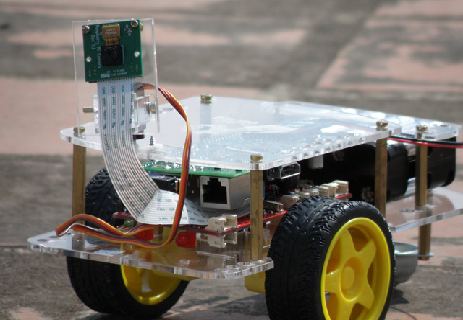
\includegraphics[width=\textwidth]{GoPiGo.png}
             \caption{GoPiGo}
             \label{fig:GoPiGo}
     \end{subfigure}%
     ~
     \begin{subfigure}[b]{0.3\textwidth}
             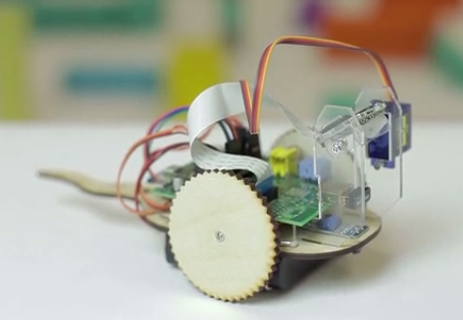
\includegraphics[width=\textwidth]{TiddlyBot.png}
             \caption{TiddlyBot}
             \label{fig:TiddlyBot}
     \end{subfigure}
     \caption{Similar educational robots}\label{fig:robots}
\end{figure}
 
\section{Project Management}

In order to have a continuous progress, project management had to be established. The goal of management is to ensure that the whole project and software development process works as it is intended, allowing project activities to meet project requirements.
\\
The main steps of project management process are initiating, planning, executing, monitoring and controlling, and closing. Thus firstly, project team meetings were established on a weekly basis. Continuing defining the project goals, tight control of timeline had to be set as well, in order to keep track of deadlines.
\\
For this purpose the Gantt charts web tool\footnote{\url{https://teamgantt.com/}} was employed. It allowed to breakdown work structure of the project to small tasks, setting the start and finish dates individually. Example of Gantt chart used in this project can be seen in figure \ref{fig:gannt_example}.

\begin{figure}[ht!]
	\centering
	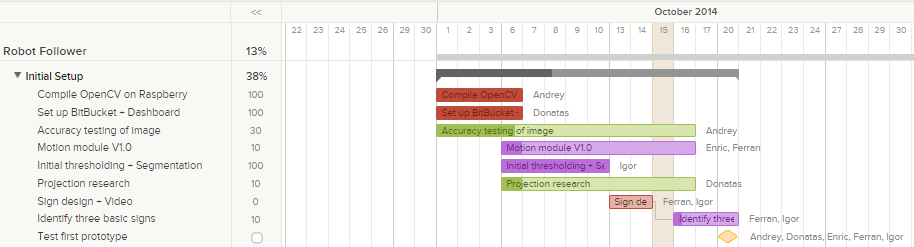
\includegraphics[width=1\textwidth]{gantt_chart_part}
	\caption{Part of planning represented on Gantt chart}
	\label{fig:gannt_example}
\end{figure}

Beside the track of the tasks, version control system for tracking the code changes had to be chosen. Common tools are Team Foundation Version Control, Mercurial or Git source control. Due to affordability and compatibility, distributed version control system Git was chosen. 
\\
For hosting the central GIT repository the two main players are \textit{Github} and \textit{Bitbucket}.
The main difference between the two is being cost for non-open source projects. \textit{Bitbucket} is free for teams up to 5 users and can host private closed source repositories whereas \textit{Github} does not provide private repositories for free. Thus the specifications of providers led to choose \textit{Bitbucket} for being web-based hosting service for this project.
\\
After setting up source version control, actual developing had started. In order to keep track with the Gantt chart, specific issues were created and assigned to each team member on a weekly basis. Project management tool \textit{Bitbucket Cards}, a part of \textit{Bitbucket}, offered interaction with issues on one easy-to-use, intuitive dashboard, where progress of tasks from one list to the next was easy to track.  Example of early stage project board can be seen in figure \ref{fig:bitcards}.

\begin{figure}[ht!]
	\centering
	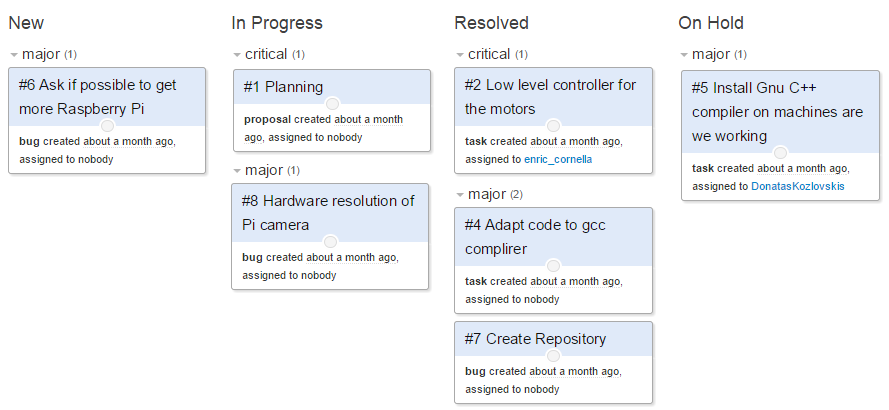
\includegraphics[width=0.7\textwidth]{bitbucket_cards}
	\caption{Early stage project board}
	\label{fig:bitcards}
\end{figure}

All mentioned tools were employed until the end of the project, resulting on continuous envelopment and progress.

\section{Implementation}
\subsection{Overview}

In this section an overview of the logic and the components which compose the system are introduced since they are explain in detail in the following sections. 

Basically, the platform has been design in a modular way and it is composed of the State manager, the vision, motion and input/output modules that interact with the different sensors, actuators and boards as it is shown in figure \ref{fig:components}.

\begin{figure}[h!]
\centering
	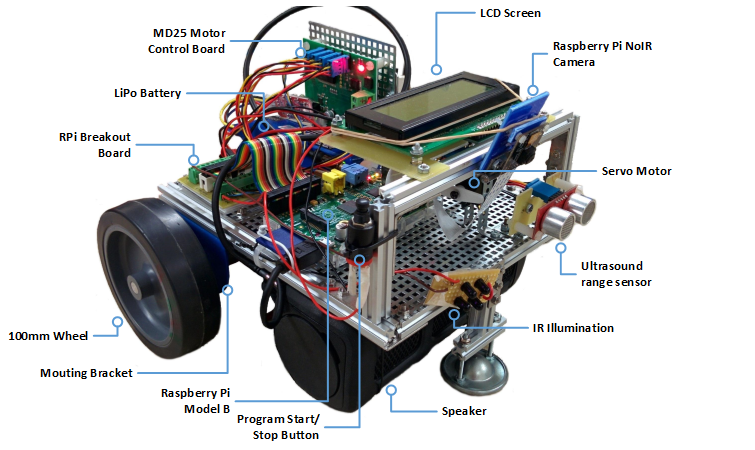
\includegraphics[width=0.8\textwidth]{robot.png}
	\caption{Overview of the robot's components}
	\label{fig:components}
\end{figure}

The sensors provided are an ultrasonic proximity sensor, a Pi nearly infrared camera and a start/stop button. This camera needs some source of infrared light thus four infrared LEDs are located in the front of the the robot. Additionally, it uses an LCD display located on the top to provide visual feedback of the current state as well as a speaker located under the robot for a sound feedback.

\newpage
The most important actuators are the motors located at both sides of the platform controlled by a MD25 motor control board as well as the servomotor that if it is necessary, can be configured in order to control the angle of vision of the NIR camera.

Moving to the logic part (figure \ref{fig:overview}), the state manager sets the current state of the robot according to the proximity sensor but mainly based on the information coming from the vision module which directly interacts with the PiCamera. The vision module carries out the analysis of the images being able to segment the scene and extract the position of the sings on the floor. It strongly uses the OpenCV library to perform this task running on the Raspberry Pi. 

\begin{figure}[h!]
     \centering
     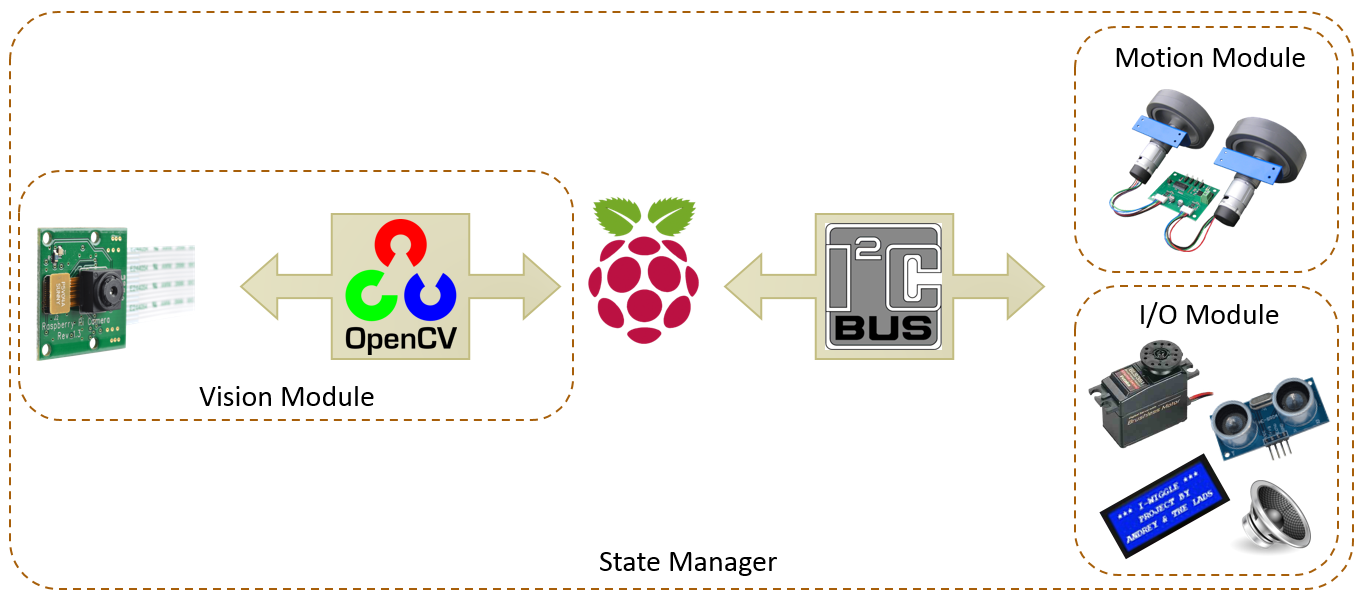
\includegraphics[width=0.7\textwidth]{overview.png}
     \caption{System overview}
     \label{fig:overview}
\end{figure}

Once a sign is detected, for instance, the state manager switches the current state acting over the motion module which controls the two motors providing the proper angular and linear speeds. The way both, the motion and the input/output module interact with the board is through the $I^2C$ bus enabled in Raspberry Pi.

On the other hand, the input/output module as its name describes, provides visual and sound feedback to the current state of the system enhancing the communication with the user.


\begin{figure}[h!]
\centering
	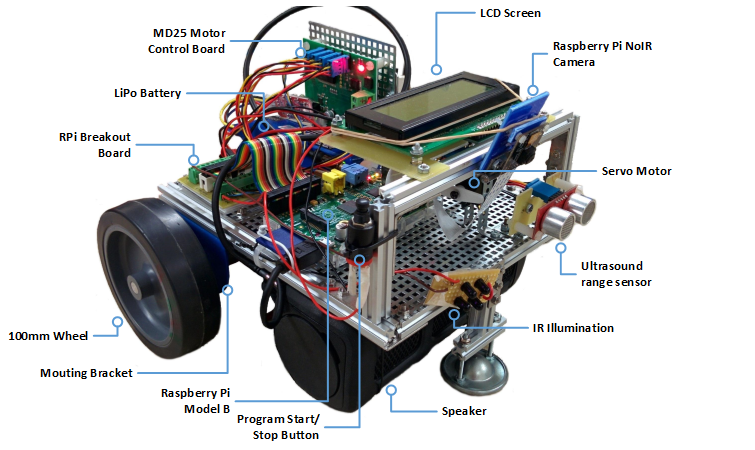
\includegraphics[width=\textwidth]{robot.png}

\caption{Overview of the robot's components}
\label{fig:overview}
\end{figure}


\subsection{Hardware}

The list of robot's main hardware components:

\begin{itemize}
  \item Raspberry Pi Model B Board
  \item Raspberry Pi No-IR Camera
  \item 2xEMG30 12v motor with encoder and 30:1 gearbox + mounting bracket
  \item Ultrasound Proximity sensor
  \item I2C Breakout Board
\end{itemize}

Insert images of the components (?).

\subsection*{Mechanical Part}

The robot is built on a metal frame with two driving wheels mounted on a EMG30
gearbox connected to the frame using the gearbox bracket. A metal ball wheel
located in front of the robot provides additional support. The frame consists of
metal profiles with a perforated plate that serves as a base for mounting
electronic components.

EMG30 is a module that incorporates motor, gearbox and encoder with Hall sensor
and suited for medium robotics applications. The gearbox provides increased
torque allowing robust movement in different environments while the Hall sensor
obtains information about the rotation of the shaft. (Include a reference to
the EMG30).



 

\subsection*{Electronics}

The main electronic component of the robot is the Raspberry Pi single-board
computer. Its technical specifications are listed in the Table
\ref{tab:rpi_specs}.

\begin{table}[h!]
	\setlength\extrarowheight{2pt}
    \begin{tabularx}{\textwidth}{XX}
    
    ~                 & ~                                                           \\
    System on a chip  & Broadcom BCM2835                                            \\
    CPU               & 700 MHz ARM11                                               \\
    GPU               & Broadcom VideoCore IV @ 250 MHz                             \\
    RAM               & 512 Mb shared with GPU                                      \\
    Memory            & SD Card Slot                                                \\
    Ports             & 2x USB, LAN, 3.5mm phone jack, HDMI,  GPIO (UART, I2C, SPI) \\
    Power Consumption & 700 mA (3.5 W)                                              \\
    
    \end{tabularx}
    \caption{Raspberry Pi Model B Specifications}
    \label{tab:rpi_specs}
\end{table}


The board is powered using 11.1V Turnigy LiPo Battery via power adapter that
splits the voltage into 12V (motors) and 5V lines. According to the external
power supply measurements, the average total consumption during movement is
(insert here).

The Raspberry Pi peripherals include a WiFi adapter, GPIO Breakout board for
simplifying connection, and a Raspberry Pi camera. RPi camera is a
board-specific 5Mp camera module connected via 15-pin MIPI (Mobile Industry
Processor Interface) connector. It is capable of capturing 1080p video and
perform basic hardware video processing. Two different types of cameras were
tested - standard camera and near-IR ``NoIR'' camera with the absence of
infrared filter. The performance of these cameras compared to standard USB
Webcam is shown in the Table \ref{tab:cam_perf}. In order to
increase the reliability and robustness of NoIR camera, a couple of IR LEDs were
installed to provide additional illumination.

Talk about sign design for the near-IR camera here.
After a series of experiments, a highly-reflective duct tape was chosen as a
material for the signs. It showed high reflectance under poor lighting
conditions. The usage of the NoIR camera accompanied with a couple of IR LEDs
showed high segmentation performance with minimum lighting provided.

MD25 is a dual H-Bridge I2C / Serial motor driver suited for the control of
EMG30 modules.
It provides additional capabilities in the motor manipulation, such as variable
acceleration, motor current information and independent control of two motors
with encoder feedback. It is also equipped with a 5V regulator, however it is
impossible to power the Raspberry Pi as the continuous supply rate is 300 mA,
while the average consumption of Raspberry Pi is 700 mA.

Put the reference.
\url{http://www.pishrobot.com/files/products/datasheets/md25.pdf}

Due to the reason explained before, Raspberry Pi is powered using Taco Power TSR
1-2450 DC-DC voltage step-down modules that provide 5V 1A output.

Put the reference.
\url{http://www.adafruit.com/datasheets/tsr1.pdf}

% Fix table here
\begin{table}[h!]
	\setlength\extrarowheight{2pt}
	\setlength\arraycolsep{5pt}
    \begin{tabularx}{\textwidth}{XXXX}
    Resolution / Camera Setup & Raspberry Pi  (CPU) + Raspberry Pi Camera &
    Raspberry Pi (CPU) + Logitech C270 & Odroid-U3 (CPU) + Logitech C270 \\
    160x120            & 18           & 9          & 30         \\
    320x240            & 6            & 4.8        & 20         \\
    640x480            & 2.5          & 2.3        & 11         \\
    1280x720           & 0.6          & 0.8        & 4          \\
    \end{tabularx}
    \caption{Camera Performance comparison}
    \label{tab:cam_perf}
\end{table}

As can be seen from the Table \ref{tab:cam_perf}, the main advantage of using
RPi camera is its performance - it outperforms generic Webcam grace to hardware
optimization and, in particular, absence of resizing routine in the code.
However, the disadvantage lies in the specificity of the camera, that can only
be used on the RPi board, while the USB Webcam can be used everywhere, so in
order to port the code to another platform, the camera change as well as some
code modification are required.

The robot is also equipped with an ultrasound proximity sensor used for obstacle
detection. It is a basic proximity sensor with a focus of 15 degrees and an
accuracy about 2mm. 

An I2C LCD Screen module provides an interface for visual feedback.
	
\subsection{Software}


Conceptual overview of software architecture and its parts is given on figure below. All components will be discussed and described in detail in this section of the report. 

\begin{figure}[th!]
\center
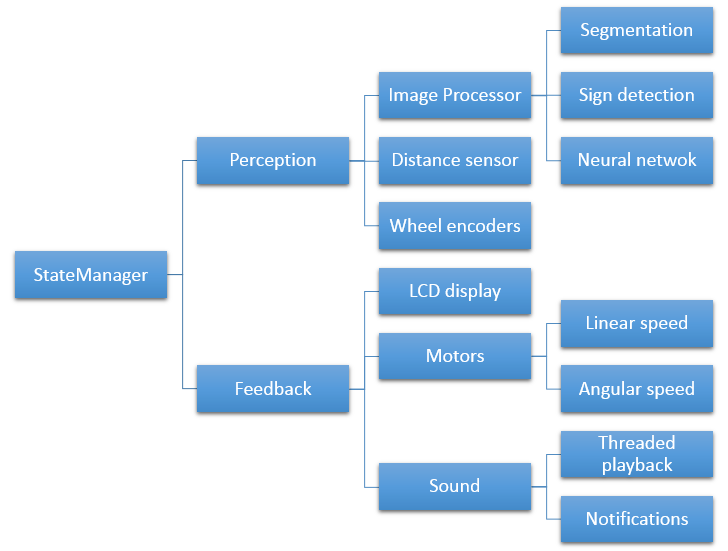
\includegraphics[scale=0.7]{images/software-architecture.png}
\caption{Overview of software architecture of the solution}
\end{figure}




\subsubsection{State machine}


One of the most common and intuitive approaches for implementation of software controller for hardware system is state-machine approach. It is fairly simple concept, with only a couple of important considerations.

System controlled by state machine has certain number of possible, unique and well defined states that it can be in at every moment of execution. State defines the behaviour of the system in every discrete moment of time, including three important aspects: sensor data acquisition, output behaviour computation and state transition check. In other words, every state has it is own logic for doing all of these three mentioned steps, which gives a lot of variability for possible control scenarios. It is worth mentioning that some states might skip certain steps or perform some steps more than once without state transition check, for example.

\paragraph{System states}

At any moment of time robot can be in one of the following state:

\begin{itemize}
	\item IDLE
	\item WIGGLING
	\item APPROACHING\_SIGN
	\item EXECUTING\_COMMAND
	\item MARCHING\_FORWARD
	\item GAME\_OVER 
\end{itemize}

\textbf{IDLE} state sets both angular and linear speed to zero and waits for any of the segmented object currently inside view to go away, after which it goes to WIGGLING state.

\textbf{WIGGLING} state rotates the robot around its vertical axis with constant angular and zero linear speed until a sign is detected. After detecting a sign it switches to APPROACHING\_SIGN state.

\textbf{APPROACHING\_SIGN} state moves the robot close to the sign it has seen in the previous state. It does this by setting the linear speed to constant value and adjusting angular speed all the time based on the horizontal position of the target sign in the view. Robot will move in the direction needed to align the sign to the center of the screen, and it will do that proportionally to the distance of the target to the center.

\textbf{EXECUTING\_COMMAND} state has different behavior depending on the type of the sign that was seen in the state before. If it was goal sign, it will switch to the GAME\_OVER state and the game will end. If it was stop sign, robot will just wait for certain predefined time-out (5 seconds) and switch to state MARCHING\_FORWARD. If it was the arrow sign, robot will turn desired angle and switch switch to state MARCHING\_FORWARD.

\textbf{MARCHING\_FORWARD} state sets the linear speed to constant and angular to zero. In this state robot constantly monitors camera image stream and can potentially switch to APPROACHING\_SIGN state once a sign is detected in perceptive area of the image.

\textbf{GAME\_OVER} state is entered after goal sign is approached. After displacing notification about game completion (through audio and visual feedback), robot remains idle until hardware button is pressed for the start of the new game.

\begin{figure}[th!]
	\centering
	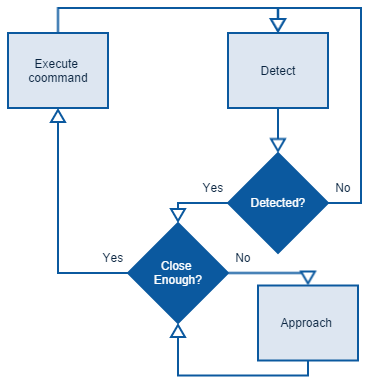
\includegraphics[scale=1]{algorithm-diagram.png}
	\caption{State transition algorithm}
	\label{fig:algorithm-diagram}
\end{figure}

\paragraph{Sensor data acquisition}

First step in state machine control loop is sensor acquisition step. If possible, data is acquired from all input sensors in order to determine current state of the environment. This includes acquisition of camera image using OpenCV, reading heading angle from motor driver and reading distances from ultrasonic sensor driver.

Last values of all the readings are always stored in local members of the class, so they can be referenced between successive acquisitions.

\paragraph{Output behavior computation}

Based on the sensed input data values for all output units are being calculated. This includes linear and angular wheel velocities, message for LCD display, sound to be played on speakers, etc.

\paragraph{State transition condition}

Every state has to have clearly defined condition which will make the system switch to any of the other states. System remains in the current state until one of the state transition conditions has been met.





\subsubsection{Actuators and sensing drivers}
Most of the processes the robot is doing need either to get some information from external sensors or to send data to the actuators or displays. This is useful in the two ways of the communication. Sensors will give information to the robot so it can sense better the environment and act in consequence of what is happening in the \textit{exterior} world. Actuators, or output peripherals, give feedback to the persons interacting with the robot. A clear example would be explaining some instructions in an LCD screen or playing some sounds in certain actions of the robot. This will make the interaction easier and enrich the experience. Whenever it is needed to communicate with external devices, the robot needs to use drivers.

Next, the sound and LCD modules are explained as output devices and ultrasonic sensor and the push button as input device. It is important to remark that, although the motion module is run using drivers, it will not be explained in this section since a special part is dedicated to it due its importance.

A driver is non other than a small program that allows a computer (in the current case a Raspberry Pi) to communicate with some external devices. It gives basic instructions and functions to make an easy interaction between the both parts.

In this point it is important to remark two different groups of devices. The first one includes the sound module, which is already built in the Raspberry Pi making it easy to connect by simply plugging a speaker using a 3.5mm jack. It also includes the push button, wired directly to the GPIO. The second group, formed by the ultrasonic sensor and the LCD screen need an $I^{2}C$ protocol in order to communicate with the RPi.

For the first group it is needed an external speaker that can be easily plugged with a standard jack. In this case the Raspberry Pi already provides support for launching different sounds so it is straight forward to make it work. A button is also wired to the RPi in order to make an easy interaction when it is needed to start or stop the program without connecting the robot to a computer or external screen. 

The button is controlled by a \textit{Python} script that is initialized manually. When this program is running it will be constantly executed. Actually the program does nothing, it simply waits until a \textit{flag} is activated due to interaction with the button. It is connected to the GPIO of the RPi in \textit{normally open} mode, closing the circuit when it is pressed.

For giving an example of how this two parts work together, whenever the button of the robot is pressed a sound is played in order to give feedback to the children about the starting or shutting down of the program. The script receives a \textit{flag} that the button has been pushed and an instruction like \textit{os.system('omxplayer sound.mp3')} reproduces a sound. In figure \ref{fig:module1} it is possible to observe how the button and speaker are connected to the Raspberry Pi. The ports used for the button are the pin number 24 and any \textit{GND}.

\begin{figure}[h]
\centering
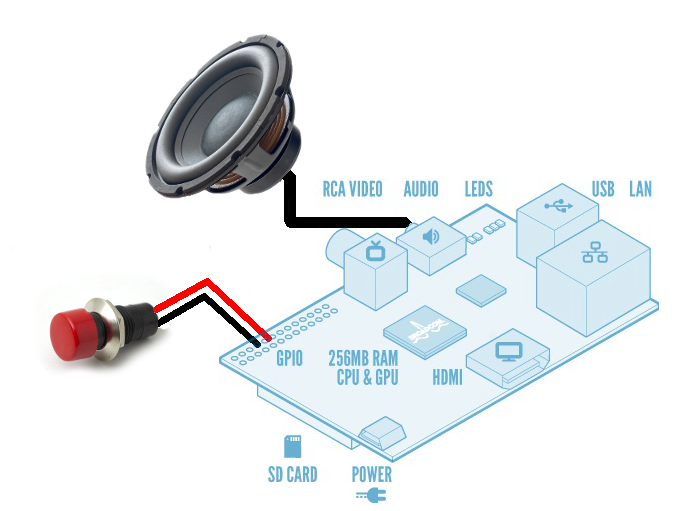
\includegraphics[width = 0.6\textwidth]{module1}
\caption{Connection of the external speaker and the button}
\label{fig:module1}
\end{figure}

In the second group a new protocol is introduced: $I^{2}C$, that refers to \textit{Inter Integrated Circuit}, a multi-master and multi-slave serial bus. It is a protocol used for attaching low-speed peripherals to embedded systems, small computers or microchips. The power of $I^{2}C$ is that allows to connect several devices in the same line of cables. By identifying each one of this devices with an unique address it is possible to control all of them. In figure \ref{fig:i2c} it is possible to observe the connection of the two devices that make use of $I^{2}C$. As can be seen only four cables are needed for sending and receiving data. Red and black are used as power source, typically +5V or +3.3V. Green and blue cables are Serial Data Line (SDA) and Serial Clock Line (SCL). The working principle of $I^{2}C$ is very simple. Each one of the devices has a specific address which is known a priori (certain addresses are available to chose for each device). When it is needed to communicate with one of them a buffer is sent to the correspondent address and the device acts in consequence. Later it is explained each one how it works.

\begin{figure}[h]
\centering
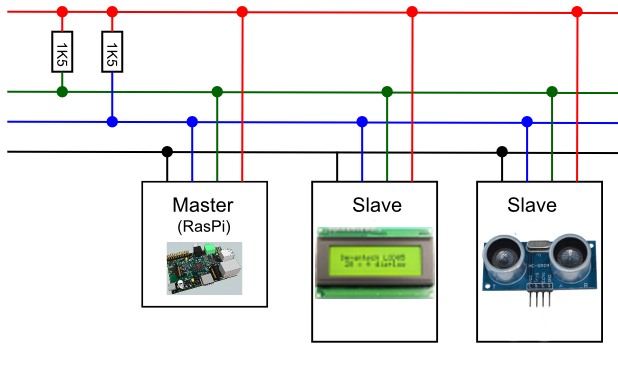
\includegraphics[width = 0.6\textwidth]{i2c}
\caption{Connection of multiple devices to a $I^{2}C$ port. Raspberry Pi is working as master while the other two peripherals are working as slave.}
\label{fig:i2c}
\end{figure}


The LCD display is used to show information about the current state of the robot. It is a very powerful way to know what the robot is thinking or doing without the need of connecting a screen to the Raspberry Pi. This is very important since the less computational power expended on the RPi the better. Avoiding the initialization of a graphical user interface will result in a slightly more fast execution of the program, which is desired. It is also a very nice way to communicate with children and explain maybe some instructions or the current state of the robot so they know what the robot is doing. The flow of the information in the $I^{2}C$ bus is only in one way, from the RPi to the LCD. Whenever it is needed to write something in the screen a command is sent via the bus and the device executes it. The two most common functions used are the ones to write and clean the screen.

The proximity sensor provides information to the robot about its surroundings. The working principle is based on ultrasonic sounds that rebound on objects. By calculating the amount of time for a sound wave to get back to the sensor it is possible to estimate the distance. In this case the $I^{2}C$ bus is working in two directions. In order to get data from the sensor first it is need to send some information to it. It is like a conversation where the RPi asks for information and the ultrasonic sensor responds with this data.In this way it is avoided to continuously receive unnecessary data. Grabbing distance two or three times per second is enough in the current case since the robot is not moving fast.


\subsubsection{Motion module}
This module connects desired action behaviour via the control of  robot wheels. Since designed robot uses
Dual 12Volt 2.8Amp H Bridge Motor Drive MD25 \footnote{\url{http://www.robot-electronics.co.uk/htm/md25i2c.htm}} board, controlling the wheels was accomplished using $I^2C$ bus system mode.
Generally this module had to realize following actions:
\begin{itemize}
	\item drive motors by setting individual speeds for both wheels;
	\item get heading of the robot by reading encoder values.
\end{itemize}
These requirements led to splitting the whole module into two blocks:  one being responsible for driving motors and another for reading/writing encoders.

\begin{figure}[!ht]
	\centering
	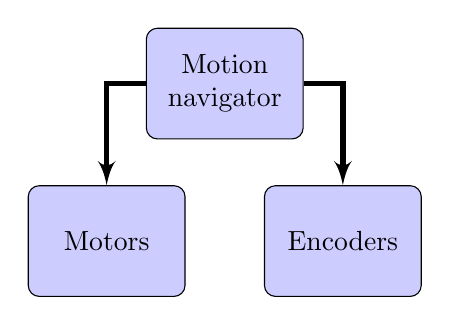
\begin{tikzpicture}[node distance = 2cm, auto]
	\tikzstyle{block} = [rectangle, draw, fill=blue!20, 
	text width=5em, text centered, rounded corners, minimum height=4em]
	\tikzstyle{line} = [draw, -latex', line width =2pt]
	% Place nodes
	\node [block] (navigator) {Motion navigator};
	\node [block, below of=navigator, xshift=-1.5cm] (motors) {Motors};
	\node [block, below of=navigator, xshift= 1.5cm] (encoders) {Encoders};
	% Draw edges
	\path [line] (navigator) -| (motors);
	\path [line] (navigator) -| (encoders);
	\end{tikzpicture}
	\caption{Motion module structure}
	\label{fig:motion_structure}
\end{figure}

\paragraph{Controlling motors}

All communications between high level functions and motors were realized via  $I^2C$ bus command register.
The MD25 has 17 registers numbered 0 to 16 as follows:
\begin{table}[!h]
	\begin{tabular}{@{}llll@{}}
		\toprule
		\textbf{Register} & \textbf{Name}     & \textbf{Read/Write} & \textbf{Description}                                             \\ \midrule
		0                 & Speed1            & R/W                 & Motor1 speed (mode 0,1) or speed (mode 2,3)                      \\
		1                 & Speed2/Turn       & R/W                 & Motor2 speed (mode 0,1) or turn (mode 2,3)                       \\
		2                 & Enc1a             & Read only           & Encoder 1 position, 1st byte (highest),   \\
		3                 & Enc1b             & Read only           & Encoder 1 position, 2nd byte                                     \\
		4                 & Enc1c             & Read only           & Encoder 1 position, 3rd byte                                     \\
		5                 & Enc1d             & Read only           & Encoder 1 position, 4th (lowest byte)                            \\
		6                 & Enc2a             & Read only           & Encoder 2 position, 1st  byte (highest),  \\
		7                 & Enc2b             & Read only           & Encoder 2 position, 2nd byte                                     \\
		8                 & Enc2c             & Read only           & Encoder 2 position, 3rd byte                                     \\
		9                 & Enc2d             & Read only           & Encoder 2 position, 4th byte (lowest byte)                       \\
		10                & Battery volts     & Read only           & The supply battery voltage                                       \\
		11                & Motor 1 current   & Read only           & The current through motor 1                                      \\
		12                & Motor 2 current   & Read only           & The current through motor 2                                      \\
		13                & Software Revision & Read only           & Software Revision Number                                         \\
		14                & Acceleration rate & R/W                 & Optional Acceleration register                                   \\
		15                & Mode              & R/W                 & Mode of operation (see below)                                    \\
		16                & Command           & Write only          & Used for reset of encoder counts and module address changes      \\ \bottomrule
	\end{tabular}
	\caption{The MD25 register values and description}
	\label{table:md25}
\end{table}

\newpage
For controlling the motors, registers 0, 1 and 15 are used. Firstly, initializing motor control, mode register (15) is modified.
The mode register selects which mode of operation and $I^2C$ data input type the user requires. Here the type 3 was chosen and writing this value 
to the mode register makes enables turn mode: "speed1" controls both motors \textit{speed}, and "speed2" becomes the \textit{turn} value. 
These two values correspond to the \textit{linear} and \textit{angular} respectively, which are provided by state machine.
Data is in the range of -128 for full reverse, 0 for stop and 127 for full forward speed of motors.

It is worth to mention, that turn mode looks at the speed register to decide if the direction is forward or reverse. Then it applies a subtraction or addition of the turn value on either motor. If the direction is forward:
\begin{table}[!ht]
	\centering
	\begin{tabular}{lcl}
		motor speed1 & = & speed - turn,\\
		motor speed2 & = & speed + turn,
	\end{tabular}
\end{table}

else the direction is reverse:
\begin{table}[!ht]
	\centering
	\begin{tabular}{lcl}
		motor speed1 & = & speed + turn,\\
		motor speed2 & = & speed - turn.
	\end{tabular}
\end{table}

Manipulating mentioned registers, 4 main motor controlling functions were implemented as shown in figure \ref{fig:motor_structure}.
\begin{figure}[!ht]
	\centering
	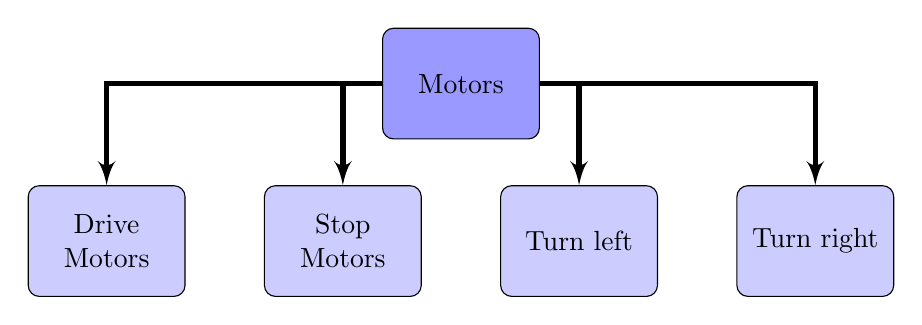
\begin{tikzpicture}[node distance = 2cm, auto]
	\tikzstyle{block} = [rectangle, draw, fill=blue!20, 
	text width=5em, text centered, rounded corners, minimum height=4em]
	\tikzstyle{line} = [draw, -latex', line width =2pt]
	% Place nodes
	\node [block,  fill=blue!40] (motors) {Motors};
	\node [block, below of=motors, xshift=-1.5cm] (stop) {Stop Motors};
	\node [block, left of=stop, node distance = 3 cm] (drive) {Drive Motors};
	\node [block, below of=motors, xshift=1.5cm] (left) {Turn left};
	\node [block, right of=left,  node distance = 3 cm] (right) {Turn right};
	% Draw edges
	\path [line] (motors) -| (drive);
	\path [line] (motors) -| (stop);
	\path [line] (motors) -| (left);
	\path [line] (motors) -| (right);
	\end{tikzpicture}
	\caption{Functions for controlling motors}
	\label{fig:motor_structure}
\end{figure}

Main function is to drive motors was implemented by sending  \textit{linear} and \textit{angular} (i.e. \textit{speed} and \textit{turn}) values, while turn functions are only using angular speed to turn around the given direction. Finally, stopping function request zero linear and zero angular speeds.

\paragraph{Controlling encoders}

For controlling the encoders, registers 2-9 and 16, listed in a table \ref{table:md25}, are used.
Manipulating mentioned registers, 3 main encoder controlling functions were implemented, which are presented figure \ref{fig:encoder_structure}.
\begin{figure}[!ht]
	\centering
	\begin{tikzpicture}[node distance = 2cm, auto]
	\tikzstyle{block} = [rectangle, draw, fill=blue!20, 
	text width=5em, text centered, rounded corners, minimum height=4em]
	\tikzstyle{line} = [draw, -latex', line width =2pt]
	% Place nodes
	\node [block, fill=blue!40] (encoders) {Encoders};
	\node [block, below of=encoders, xshift=-1.5cm] 	(rleft) {Read right encoder};
	\node [block, left of=stop, node distance = 3 cm] 	(lleft) {Read left encoder};
	\node [block, below of=encoders, xshift=1.5cm] 	(reset) {Reset both encoders};
	\node [block, right of=left,  node distance = 3 cm] (angle) {Get robot heading};
	% Draw edges
	\path [line] (encoders) -| (rleft);
	\path [line] (encoders) -| (lleft);
	\path [line] (encoders) -| (reset);
	\path [line] (encoders) -| (angle);
	\end{tikzpicture}
	\caption{Functions for manipulating encoders }
	\label{fig:encoder_structure}
\end{figure}

While getting values of encoders or resetting counts included only reading/sending the values from  $I^2C$ bus command register, robot \textit{heading} calculation is implemented realising two formulas stated in equations \ref{eq:rb_rad-pc}- \ref{eq:rb_heading},
%$$
%radiansPerCount = \pi* (wheelDiameter/trackWidth) / countsPerRevolution
%$$
%and
%$$
%heading = (countsEncoderRight - countsEncoderLeft) * radiansPerCount
%$$ 

\begin{eqnarray}
rad_{pc}  = & \pi \cdot \frac{ d_{wheel} }{ d_{track} } / c_{pr}	,
\label{eq:rb_rad-pc}
\\
\theta_{h} = & (ce_{r} - ce_{l} ) \cdot rad_{pc} ,
\label{eq:rb_heading}
\end{eqnarray}
where 
\begin{itemize}
	\item $rad_{pc}$ - radians per one encoder count,
	\item $d_{wheel}$ - wheel diameter,
	\item $d_{track}$ - track width (or distance between the wheels), %as in figure \ref{fig:rb_wheel_graph},
	\item $c_{pr}$ - encoder counts per output shaft (wheel) turn,
	\item $ce_{r}$ - right encoder counts,
	\item $ce_{l}$ - left encoder counts,
	\item $\theta_{rh}$ - robot heading in radians.
\end{itemize}

Knowing our system constant parameters from robot model shown in figure \ref{fig:rb_wheel_graph},
$$
d_{track} = 224 (mm), \ d_{wheel}=100 (mm), \ c_{pr}=360,
$$
radians per one encoder count can be expressed as
$$
rad_{pc}  = \frac{\pi}{360}\cdot \frac{ 100 }{ 224 } = \frac{\pi}{180}\cdot \frac{ 50 }{ 224 }.
$$

\begin{figure}[!ht]
	\centering
	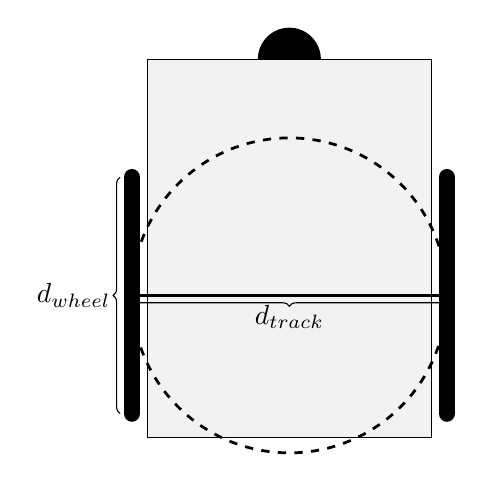
\begin{tikzpicture}
	\def\whDist{2}
	\def\whRad{1.5}
	\def\thirdWheel{3}
	\def\rectBound{0.3}
	
	% wheels
	\draw[line width=6pt, line cap=round] (-\whDist, -\whRad) -- (-\whDist, \whRad);
	\draw[line width=6pt, line cap=round] (\whDist, -\whRad) -- ( \whDist, \whRad);
	%third wheel circle
	\fill[line width = 1pt]  (0, \thirdWheel) circle (0.4);
	
	%robot box
	\draw[fill=gray!10] (-\whDist+0.2, -\whRad-\rectBound) rectangle (\whDist-0.2, \thirdWheel);
	
	% robot circle
	\draw[line width = 1pt, dashed]  (0, 0) circle (\whDist);
	
	%axis between wheels
	\draw[line width = 1pt]  (-\whDist, 0) -- (\whDist, 0);
	%distance decoration
	\draw[ decoration={brace}, decorate] (-\whDist-0.15, -\whRad) -- (-\whDist-0.15, \whRad) node[pos=0.5, anchor=east, ] {$d_{wheel}$};
	%wheel decoration
	\draw[ decoration={brace, mirror, raise=0.05cm}, decorate] (-\whDist, 0) -- (\whDist, 0) node[pos=0.5, anchor=north] {$d_{track}$};
	
	\end{tikzpicture}
	\caption{Robot wheel positioning}
	\label{fig:rb_wheel_graph}
\end{figure}
% optional new page
% to adjust figure
Assuming that our requirement is angle in degrees
$$
\theta_{dh} =  \frac{180}{\pi} \theta_{rh},   
$$
equation \ref{eq:rb_heading} can be simplified and robot heading in degrees can be calculated as
\begin{align*}
\theta_{dh} 
& = \frac{180}{\pi} (ce_{r} - ce_{l} ) \cdot rad_{pc} 								\\
& = \frac{180}{\pi} (ce_{r} - ce_{l} )   \frac{\pi}{180}\cdot \frac{ 50 }{ 224 } 	\\
& = (ce_{r} - ce_{l} ) \cdot \frac{ 50 }{ 224 } 									\\
& \Longrightarrow \\
\theta_{dh}
& = (ce_{r} - ce_{l} ) \cdot \frac{ d_{wheel} }{ 2\cdot d_{track} } .
\end{align*}

Having the left and right encoder counts, the latter equation enable to estimate wheeled robot's heading.
\\
As one knows, dead reckoning is subject to cumulative errors, however in our case, such system position tracking is not implemented. And long-time accumulative errors do not affect turning robot the requested angle, since not the actual accumulative encoder values are used, but only the difference between encoder counts before requesting an action and after.



\subsubsection{Vision module}

The task of vision subsystem is to handle the image data acquired from Raspbery Pi camera. This handling includes two basic subtasks: sign detection and sign recognition (classification).

Three basic signs detected and recognized by the system are shown on figure \ref{fig:raw-signs}. They are printed on a flat paper surface.

\begin{figure}[th!]
	\centering
	\begin{subfigure}[b]{0.2\textwidth}
		\centering
		
\includegraphics[scale=0.25]{sign-circle.png}
		\subcaption{Circle (goal)}
	\end{subfigure}
	\begin{subfigure}[b]{0.4\textwidth}
		\centering
		
\includegraphics[scale=0.25]{sign-arrow.png}
		\subcaption{Arrow (direction change)}
	\end{subfigure}
	\begin{subfigure}[b]{0.2\textwidth}
		\centering
		
\includegraphics[scale=0.25]{sign-cross.png}
		\subcaption{Cross (stop)}
	\end{subfigure}
	\caption{Shape of signs used by the system}
	\label{fig:raw-signs}
\end{figure}

Basic workflow of the vision processing module is split into functional blocks, shown on the figure \ref{fig:vision-module-blocks}.

%\begin{figure}[th!]
%	\centering
%		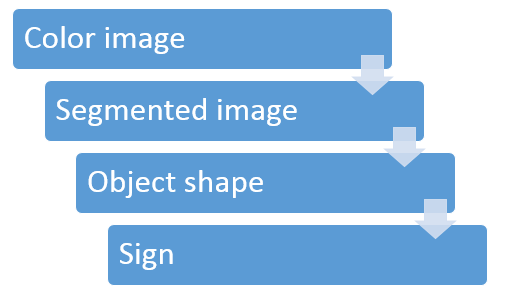
\includegraphics[scale=0.5]{image-module.png}
%	\caption{Workflow of vision module}
%	\label{fig:vision-module-blocks}
%\end{figure}

\begin{figure}[!ht]
	\centering
	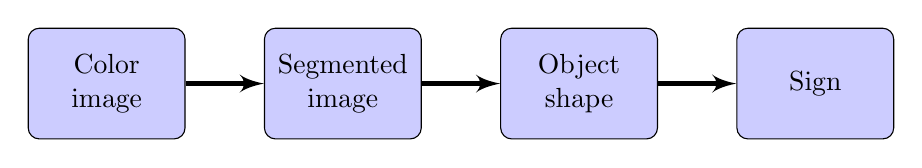
\begin{tikzpicture}[node distance = 2cm, auto]
	\tikzstyle{block} = [rectangle, draw, fill=blue!20, 
	text width=5em, text centered, rounded corners, minimum height=4em]
	\tikzstyle{line} = [draw, -latex', line width =2pt]
	% Place nodes
	\node [block] (ci) {Color image};
	\node [block, right of=ci, node distance = 3 cm] (si) {Segmented image};
	\node [block, right of=si, node distance = 3 cm] (os) {Object shape};
	\node [block, right of=os, node distance = 3 cm] (sign) {Sign};
	% Draw edges
	\path [line] (ci) -- (si);
	\path [line] (si) -- (os);
	\path [line] (os) -- (sign);
	\end{tikzpicture}
	\caption{Workflow of vision module}
	\label{fig:vision-module-blocks}
\end{figure}




Different methods and challenges encountered in vision module are described and discussed separately in the following chapters of the report.
\paragraph{Inverse Perspective Mapping}

In this project, a single camera mounted in the front of the robot with small tilting angle is used to capture the images. Since object of interest are found on a ground plane, before applying any image recognition and classification methods, it is common-sense to process obtained camera images using Inverse Perspective Mapping (IPM).
Knowing that camera tilting angle and position on the robot is fixed, this transform is just a  plane-to-plane homography to convert the perspective image to
top view to the ground plane image. The IPM can be applied to all three planes of colour image separately or only on selected colour plane. Example of the transform can be seen in figure \ref{fig:ipm_example}.
\begin{figure}[!ht]
	\centering
	\begin{subfigure}[b]{0.3\textwidth}
		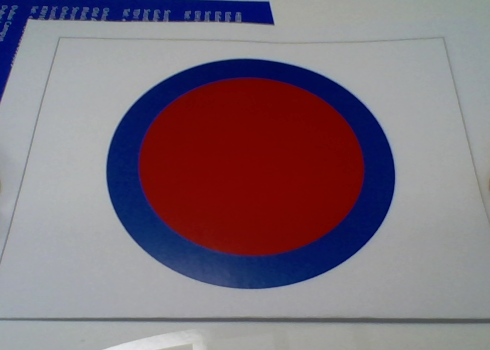
\includegraphics[width = 1\textwidth]{invPersInput.png}
		\caption{Robot captured image}
		\label{fig:}
	\end{subfigure}%
	~ 
	\begin{subfigure}[b]{0.3\textwidth}
		
\includegraphics[width = 1\textwidth]{invPersOutput.png}
		\caption{Output image after IPM}
		\label{fig:}
	\end{subfigure}
	%main caption
	\caption{Example of Inverse Perspective Mapping on a single colour image plane}
	\label{fig:ipm_example}
\end{figure}

\paragraph{Thresholding}

The first and the most intuitive approach to sign detection procedure was simple color thresholding, since signs which had to be detected are purely red.

The initial choice for color thresholding was HSV color space. Ranges of H (hue), S (saturation) and V (value) channels are [0,180], [0, 255] and [0, 255], respectively. In order to segment only red color, values of H (hue) channel greater than 170 and lower than 10 were used, since this range represents the band of red color. Additionally, too dark (V $ < $ 40), to bright (V $ > $ 220) and non-saturated pixels (S $ < $ 40) were rejected to improve the quality of segmentation. Results are shown on the figure ~\ref{fig:color-spaces}.

\begin{figure}[th!]
	\centering
	\begin{subfigure}[b]{0.3\textwidth}
		\centering
	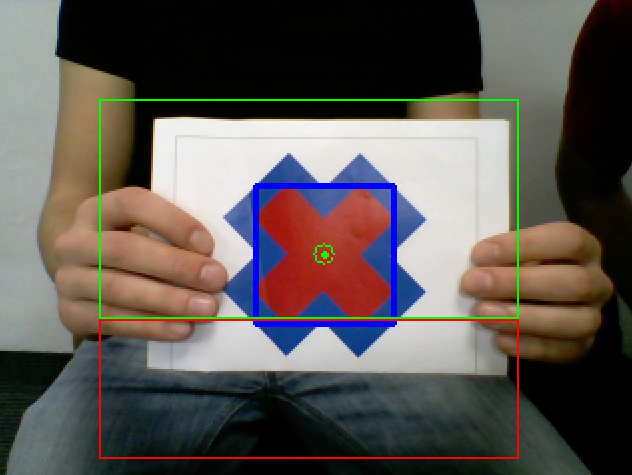
\includegraphics[scale=0.33]{thresholding-raw.png}
	\subcaption{Raw camera input}
	\end{subfigure}
	\begin{subfigure}[b]{0.3\textwidth}
		\centering
		
\includegraphics[scale=0.7]{thresholding-hsv.png}
		\subcaption{HSV color space}
	\end{subfigure}
	\begin{subfigure}[b]{0.3\textwidth}
		\centering
		\includegraphics[scale=0.7]{thresholding-YCrCb.png}
		\subcaption{YCrCb color space}
	\end{subfigure}
	\caption{Comparison of color spaces used for thresholding}
	\label{fig:color-spaces}
\end{figure}

After some testing, YCrCb color space proved to give better results for segmentation, as shown on figure above. As a result, YCrCb colour space was used in final implementation.

Usage of IR camera did not affect the recognition quality of the thresholding procedure in regular, normal lighting conditions. On the other hand, it drastically increased the accuracy in low lighting conditions, which is described in Hardware section of the report.

The biggest connected component (blob) in the thresholded image is considered to be a sign. Bounding box of the biggest blob determined the area of the thresholded image to be passed in as an input to the sign classification module. 

\paragraph{Classification of the signs using statistical moments}

Taking into consideration the relatively low computational power of the hardware platform used to develop the system, priority for the chosen sign classification algorithm was low complexity.

After some thorough analysis of the available option, statistical moments proven to be the best option.

For an arbitrary binary (i.e. thresholded) input image system can compute statistical moments of desired order. The moment of importance in case of sign classification was center of mass or first order moment. It can be thought of average coordinate of all white pixels for both axes.

\begin{figure}[th!]
	\centering
	\begin{subfigure}[b]{0.25\textwidth}
		\centering
		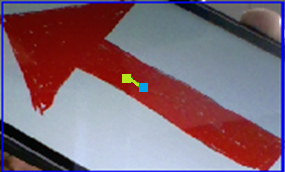
\includegraphics[scale=0.55]{moments-arrow-raw.png}
		\subcaption{Raw camera input}
	\end{subfigure}
	\begin{subfigure}[b]{0.25\textwidth}
		\centering
		
\includegraphics[scale=0.8]{moments-arrow-segm.png}
		\subcaption{Arrow}
	\end{subfigure}
	\begin{subfigure}[b]{0.2\textwidth}
		\centering
		
\includegraphics[scale=0.8]{moments-cross-segm.png}
		\subcaption{Cross}
	\end{subfigure}
	\begin{subfigure}[b]{0.2\textwidth}
		\centering
		
\includegraphics[scale=0.9]{moments-circle-segm.png}
		\subcaption{Circle}
	\end{subfigure}
	\caption{Visual cues for sign classification using statistical moments}
	\label{fig:statistical-moments}
\end{figure}

Figure \ref{fig:statistical-moments} demonstrates intuition behind visual cues used for discrimination of three different types of signs. By computing the distance of center of the mass (green rectangle) and center of the cropped image segment where the sign was detected (blue rectangle) we can perform initial discrimination between \textbf{arrow} and \textbf{rest two signs}. Distance is going to be close to zero in case of cross and circle since object are symmetrical around two mutually normal axes. Arrow is not symmetrical around one axis, so it's center of the mass will be slightly shifter towards the tip of the arrow and this is the property used to distinguish an arrow from the circle and cross.
Table \ref{tab:moments} shows average distance of center of the mass from image center proportional to cropped image size. Clear observation is that thresholding this distance to 10 $\%$ can give is pretty good estimate of probability that sign belongs to arrow class.

If this distance is close to zero, additional step is needed to determine is the observed sign cross or circle. Approach used in this step was investigation of zero-order moment, which gives the number of white pixels in the image. By taking the ratio of zero order moment and total number of pixels of sign area, we can distinguish between cross and circle. Intuition behind this metric lies in the fact that circle has bigger surface than cross of the same bounding box size, so the percentage of space it occupies in the cropped image area where the sign is going to be larger than if it was cross. Table \ref{tab:moments} gives suitable value of threshold of 70 $\%$.

\begin{table}[th!]
\centering
\begin{tabular}{l*{2}{c}r}
	Sign class			& Distance of first moment & Ratio of second order moment  \\
	\hline
	Arrow 				& 18.41 & 56.44  \\
	Cross            	& 1.39 & 54.20  \\
	Circle           	& 0.97 & 89.63  \\
\end{tabular}
\caption{Numerical values of statistical moments given in $\%$ wrt. image size}
\label{tab:moments}
\end{table}

Described method proved to be sufficiently accurate for practical purposes, while still remaining \textbf{computationally tractable} on available hardware. More robust classification methods will be discussed in section \ref{sec:future-improvements} and are subject to future investigation.

\paragraph{Neural network classifier}

Justification of usage neural networks.

Very brief theoretical background.

Description of the way how we train it on images (raw pixel values, segmentation pixels, hu-moments as inputs, etc)

Description of tested recognition method (sliding window, random, ...)

Performance comparison with previous method.

\paragraph{Computing arrow orientation}

After sign has been classified as arrow, additional step needs to be performed in order to extract the arrow angle relative to the orientation of the robot at the moment of observation.

Initial idea was to use already computed information about the statistical moments to get the orientation of the arrow. Center of the mass and center of the cropped image segment containing the sign form a vector pointing towards tip of the arrow. We can exploit this information to determine the angle of the vector, as shown on figure \ref{fig:arrow-angle-computation}. Although not so robust, this was intuitive and the fastest method to prototype since all moments are already computed for sign classification step, which meant that this method would reduce computational overhead.

\begin{figure}[th!]
	\centering
	\begin{subfigure}[b]{0.45\textwidth}
		\centering
		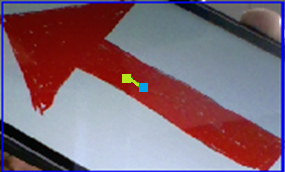
\includegraphics[scale=0.7]{moments-arrow-raw.png}
		\subcaption{Raw camera input}
	\end{subfigure}
	\begin{subfigure}[b]{0.45\textwidth}
		\centering
		
\includegraphics[scale=1]{moments-arrow-segm-angle.png}
		\subcaption{Arrow}
	\end{subfigure}
		\begin{subfigure}[b]{0.45\textwidth}
			\centering
			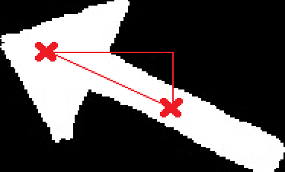
\includegraphics[scale=0.7]{moments-arrow-segm-angle-math.png}
			\subcaption{Angle from moments}
		\end{subfigure}
		\begin{subfigure}[b]{0.45\textwidth}
			\centering
			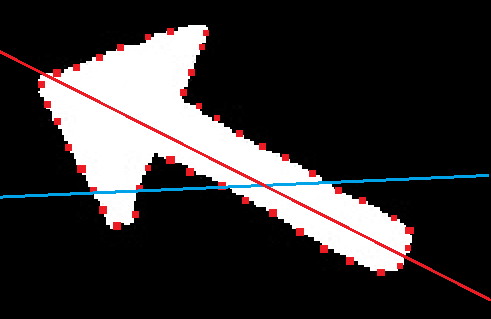
\includegraphics[scale=0.55]{moments-arrow-segm-angle-fitting.png}
			\subcaption{Line fitting}
			\label{fig:line-fitting}
		\end{subfigure}
	\caption{Computation of the arrow orientation}
	\label{fig:arrow-angle-computation}
\end{figure}

After implementation and extensive testing of mentioned method, some scenarios where it fails were met. One of them is shown in the figure , where wrong value of the angle is computed or it wasn't reliable enough (it was oscillating a lot). Oscillation problem could have been solved by filtering, but instead a different approach was chosen.

Instead of focusing on statistical properties of the contour of the arrow better approach is to utilize the whole information about it's contour. Contour of the arrow shape is extracted from segmented binary image of the arrow. Array of points representing the contour is then fitted to the line in \textbf{Linear Least Squares fashion (LLS)}, which is a well known function minimization framework for linear systems.

The basic idea is posing the problem of finding unknown arrow angle $\theta$ as function minimization problem, where input is defined as set $C$ of $N$ contour points $C_i \in \mathbb{R}^2$. Cost function on a set of points $C$ and chosen angle $\theta$ is defined as sum of the squared distance of each contour point $C_i$ from the line with angle $\theta$, which is formally given by equation \ref{eq:LLS}. Minimizing this function over $\theta$ gives the optimal line angle that fits the given contour points.

\begin{equation}
f(C,\theta)=
\frac{1}{N}
\sum_{i=1}^{N}distance(C_i, line(\theta))^2
\label{eq:LLS}
\end{equation}

Figure \ref{fig:line-fitting} shows two arbitrary lines on top of the segmented image of the arrow. Blue line has higher value of the cost function than the red line because it doesn't fit the given data (contour points) the best possible way. Red line is the optimal angle for given shape, determined by least square solution of the equation \ref{eq:LLS}.

OpenCV has LLS implementation of described line fitting algorithm, which was used in the final version of the solution. Using this method improved the accuracy and stability of orientation of the arrow without significant impact on performance, since optimization problem can be solved using techniques linear algebra, which are computationally inexpensive.

\paragraph{Solving partial occlusion and re-detection}

Problem of partial occlusion arises when robot is moving forward and a sign is slowly getting into the area observed by robot. Some time is needed before the sign completely enters the view and attempt of classification partially visible sign would result in misclassification in most of te cases.

Also, there is a problem of detecting proximity of the robot to the observed sign, because desired behavior is to switch states only when the robot is close to sign it detects and not as soon it detects it.

In order to prevent attempts of classifications of partially visible signs and detecting proximity of the robot to the sign, whole view of the camera is split into two regions of interest: \textbf{perceptive area} and \textbf{proximity area}, shown on figure \ref{fig:camera-view-areas}. Using these view areas system is able to overcome the described problems in very easy and intuitive way.

\begin{figure}[th!]
	\centering
		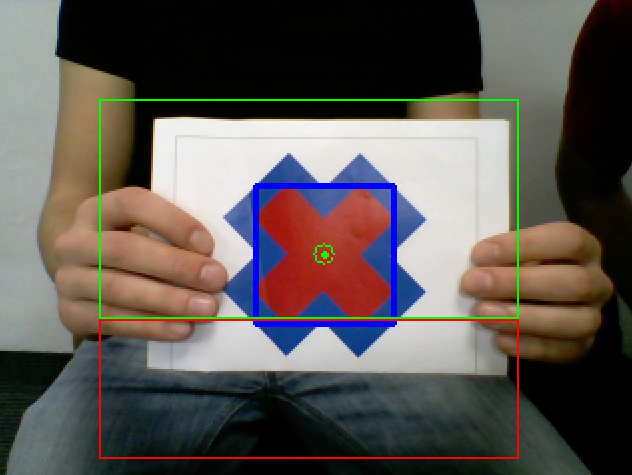
\includegraphics[scale=0.5]{thresholding-raw.png}
	\caption{Perceptive (green) and proximity (red) area}
	\label{fig:camera-view-areas}
\end{figure}

Detection of the sign (segmentation and blob detection) are performed at every iteration and position of the object is extracted as center of the detected blob. For predefined camera position and physical size of the signs, it can be assumed that \textbf{if object's center is inside the perception area it will be completely inside the camera view}. This allows reliable determination of exact classification moment, without risk of classifying partially visible objects.

Similar strategy is used for detecting the proximity of the sign: if it's center is in the proximity area it is assumed to be close to the robot. Since slightly delayed image processing and low FPS, it will take some time for robot to determine that it approached the sign. This will result in robot ending up exactly on the sign at the moment when it switches to execution of the command defined by the sign.


\section{ Final setup }
\begin{itemize}
\item
Explain the final setup of the robot. Specially the things that were not included initially (IR camera, IR leds, button to start program).
\item
Testing results.
	\begin{itemize}
	\item
	How homography helps.
	\item
	How IR helps.
	\item
	How improvement of arrow angle detection helps.
	\end{itemize}
\item
Specifications achieved (fps, missdetections, etc.)
\end{itemize}

\section{Problems encountered}


\subsection{Limitations}

The hardware of the Raspberry Pi doesn't allow to perform any intensive
computations, so it is necessary to balance between robustness and
computational time.

\subsection{Hardware}

\begin{itemize}
  	\item The overall performance of the Raspberry Pi is satisfactory. 
  	\item The reliability of the WiFi connection is low - the board can lose
  connection to WiFi dongle at any time. Loss of the connection can also be caused by an
external disturbance (e.g. sharp velocity changes).
	\item RPi Camera Module is very sensitive to static electricity.
	\item Sharp increase of the torque in the motors can cause the voltage drop in
	the power supply that will lead to board shutdown
\end{itemize}

Power plug issues (?)

\subsection{Software}

\begin{itemize}
  \item OpenCV takes almost 9 hours to compile. (Include OpenCV compilation
  guide?)
  \item No Software is available for the GPU access
\end{itemize}

It is not very convenient to develop on the Raspberry Pi itself, so it was
necessary to make the code cross-compilable. The development process was done
MS Visual Studio. Remote access to RPi is established via SSH and an xServer.
Remote Desktop Environment was provided by MobaXTerm software.

\section{Further improvements}
\label{sec:future-improvements}


\subsection{Robustness of sign classification}

Current sign classification approach is computationally inexpensive and has a simple implementation and execution. It results in low robustness, meaning that on some occasions the robot detects some other red object's shape as one of the three signs that it needs to classify.

In order to avoid these issues, a more robust classifier is required. An approach using artificial neural networks, Support Vector Machines or any other machine learning technique would require training classifiers on another (more powerful) CPU and loading the trained classifier to the robot just for the purpose of classification.

\subsection{Complex game rules and sign diversity}

Current rules for interaction with robot rely only on a couple of simple actions and available signs. Software control architecture is built in a modular way, which enables easy addition of the new signs under assumption of robust classifier able to distinguish between all currently known signs and newly added one.

Expanding set of available signs could enrich the game experience by introducing new objectives, goals and obstacles for the children to play with.

\subsection{Hardware improvements}

Although system is currently capable of performing all desired tasks, a more powerful processing hardware would make it faster, more responsive and funnier for children to play with. Having only 6 \textit{fps} from camera, limits the maximum speed of robot movement so games would look more dynamic if the robot were able to move faster. 
It would also enable usage of more advanced and, at the same time, more robust algorithms for image processing. This would remove some limitations and conditions put on the usage of the robot, like camera pointing only towards ground (floor) plane, maximum distance of sign placement, sign shape and colour restrictions, etc..
More sensors would enrich engagement of the children as well by providing diverse set of ways to interact with the robot. 




%Example of cite and referencing:\cite{craig2005introduction}

\printbibliography

\end{document}